\documentclass[12pt]{report}
\usepackage{graphicx}
\usepackage{array}
\usepackage{tabularx}
\usepackage{amsmath}
\usepackage{hyperref}
\usepackage{geometry}
\usepackage{fontspec} % For custom fonts
\usepackage{xcolor}
\usepackage{float}
\usepackage{titling}
\usepackage{tikz}
\usepackage{fancyhdr} % For custom headers/footers
\usepackage{tocbibind} % To include TOC, LOF, LOT in TOC
\setmainfont{Times New Roman} % Set the main font to Times New Roman
\geometry{a4paper, margin=1in}
\usepackage{setspace}
\onehalfspacing 
\usepackage{titlesec}
\usepackage{fancyhdr}
\usepackage[titles]{tocloft}
\usepackage{chngcntr}

\counterwithout{figure}{chapter}

\renewcommand{\cftpartpresnum}{PARTIE~} 
\renewcommand{\cftpartaftersnum}{.}     
\renewcommand{\cftpartleader}{\cftdotfill{\cftdotsep}}
\setlength{\cftpartnumwidth}{5em}

\renewcommand{\cftchappresnum}{Chapitre~}
\renewcommand{\cftchapaftersnum}{.}     
\renewcommand{\cftchapleader}{\cftdotfill{\cftdotsep}}
\setlength{\cftchapnumwidth}{5em}

\pagestyle{fancy}
\fancyhf{} % Clear all header and footer fields
\fancyfoot[C]{\thepage} % Place the page number in the center of the footer
\renewcommand{\headrulewidth}{0pt}  % Removes the line in the header
\renewcommand{\footrulewidth}{0pt}  % Removes the line in the footer
\hypersetup{
   colorlinks=true,
  linkcolor=black,   % Set link color to black
  filecolor=magenta, 
  urlcolor=cyan,
  pdfborder={0 0 0} 
}
\renewcommand{\contentsname}{SOMMAIRE GENERAL} 
\renewcommand{\listtablename}{LISTE DES TABLEAUX}
\renewcommand{\listfigurename}{LISTE DES FIGURES}
\newcommand{\figref}[1]{figure \ref{#1}}

\titleformat{\part}[display]
  {\normalfont\Huge\bfseries\centering}
  {PARTIE \Roman{part}}{20pt}{\Huge}

\titleformat{\chapter}[display]
  {\normalfont\Large\bfseries\centering}
  {Chapitre \arabic{chapter}~.}{20pt}{\Large}

\titleformat{\section}
    {\normalfont\large\bfseries} 
    {\thesection}
    {1em}
    {\large}
	
\begin{document}	
			 \pretitle{
				\begin{tikzpicture}[remember picture, overlay]
			   		\node[anchor=north west, xshift=1.5cm, yshift=-1cm] at (current page.north west) {
        						\includegraphics[width=2.5cm]{image1.png}
					};
    					\node[anchor=north west, xshift=4cm, yshift=-1cm] at (current page.north west) {
        						\includegraphics[width=2.3cm]{image2.png}
					};
					\node[anchor=north east, xshift=-1.5cm, yshift=-1cm] at (current page.north east) {
        						
\includegraphics[width=5cm]{image3.png}
					};
				\end{tikzpicture}
				\begin{center}
					\textbf{\large UNIVERSITE DE FIANARANTSOA ECOLE NATIONALE D'INFORMATIQUE \\[0.5cm] MEMOIRE DE FIN D'ETUDES POUR L'OBTENTION DU DIPLOME DE MASTER PROFESSIONNELLE}
					\\[0.5cm]
							\textbf{\underline{Mention:}} Informatique \\	
							\textbf{\underline{Parcours:}} Informatique générale\\
							\textbf{\textit{Intitulé}}				\end{center}
				\begin{center}\Large\bfseries
			}
			\preauthor{\begin{flushleft}\fontsize{12} \lineskip Présenté le 01 février 2023 }
			\postauthor{\end{flushleft} \textbf{Membres du Jury:} 
			 \begin{itemize}
			    \item \textbf{Président:} Monsieur RALAIVAO Jean Christian, Assistant d'Enseignement Supérieur et de Recherche;
			    \item \textbf{Examinateur:} Monsieur RALAIVAO Jean Christian, Assistant d'Enseignement Supérieur et de Recherche;
			    \item \textbf{Rapporteurs:} \begin{itemize}
       									 \item Monsieur RALAIVAO Jean Christian, Assistant d'Enseignement Supérieur et de Recherche;
       									 \item Monsieur RALAIVAO Jean Christian, Assistant d'Enseignement Supérieur et de Recherche.
    								\end{itemize}
			\end{itemize} }
			\predate{\begin{flushright} Année Universitaire: }
			\postdate{\end{flushright}}
			\title{
				\color{blue}
				\setlength{\fboxsep}{10pt} 
				\begin{center}
					\fbox{
						\begin{minipage}{0.95\textwidth}
							\begin{center}
								CONCEPTION ET REALISATION  D'UNE APPLICATION WEB  DE RESERVATION DE VOYAGE
							\end{center}
						  \end{minipage}
					}
				\end{center}
			}
			\author{\textbf{Par:} Monsieur ANDRIAMIORA Ainamalala Lucky}
			\date{2024-2025}
			\maketitle
			
			\newpage
			\thispagestyle{empty}
			\mbox{}

			\newpage
			\pagenumbering{roman}
			\renewcommand{\thepage}{\Roman{page}} % Ensure uppercase Roman numerals
			\setcounter{page}{1}
			\chapter*{CURRICULUM VITAE}
			\addcontentsline{toc}{chapter}{CURRICULUM VITAE}	
			\begin{minipage}{0.6\textwidth}
				\textbf{Nom:} ANDRIAMIORA\\
				\textbf{Prenom:} Ainamalala Lucky\\
				\textbf{Numéro:} +261 34 33 513 61\\
				\textbf{Addresse:} IIG20 E Ambatomaro, Antananarivo\\
				\textbf{E-mail:} luckyainamalalalucky@gmail.com\\
				\textbf{Date et lieu de naissance:} 30 décembre 1999 à Antsirabe
			\end{minipage}
			\hfill
			\begin{minipage}{0.3\textwidth}
				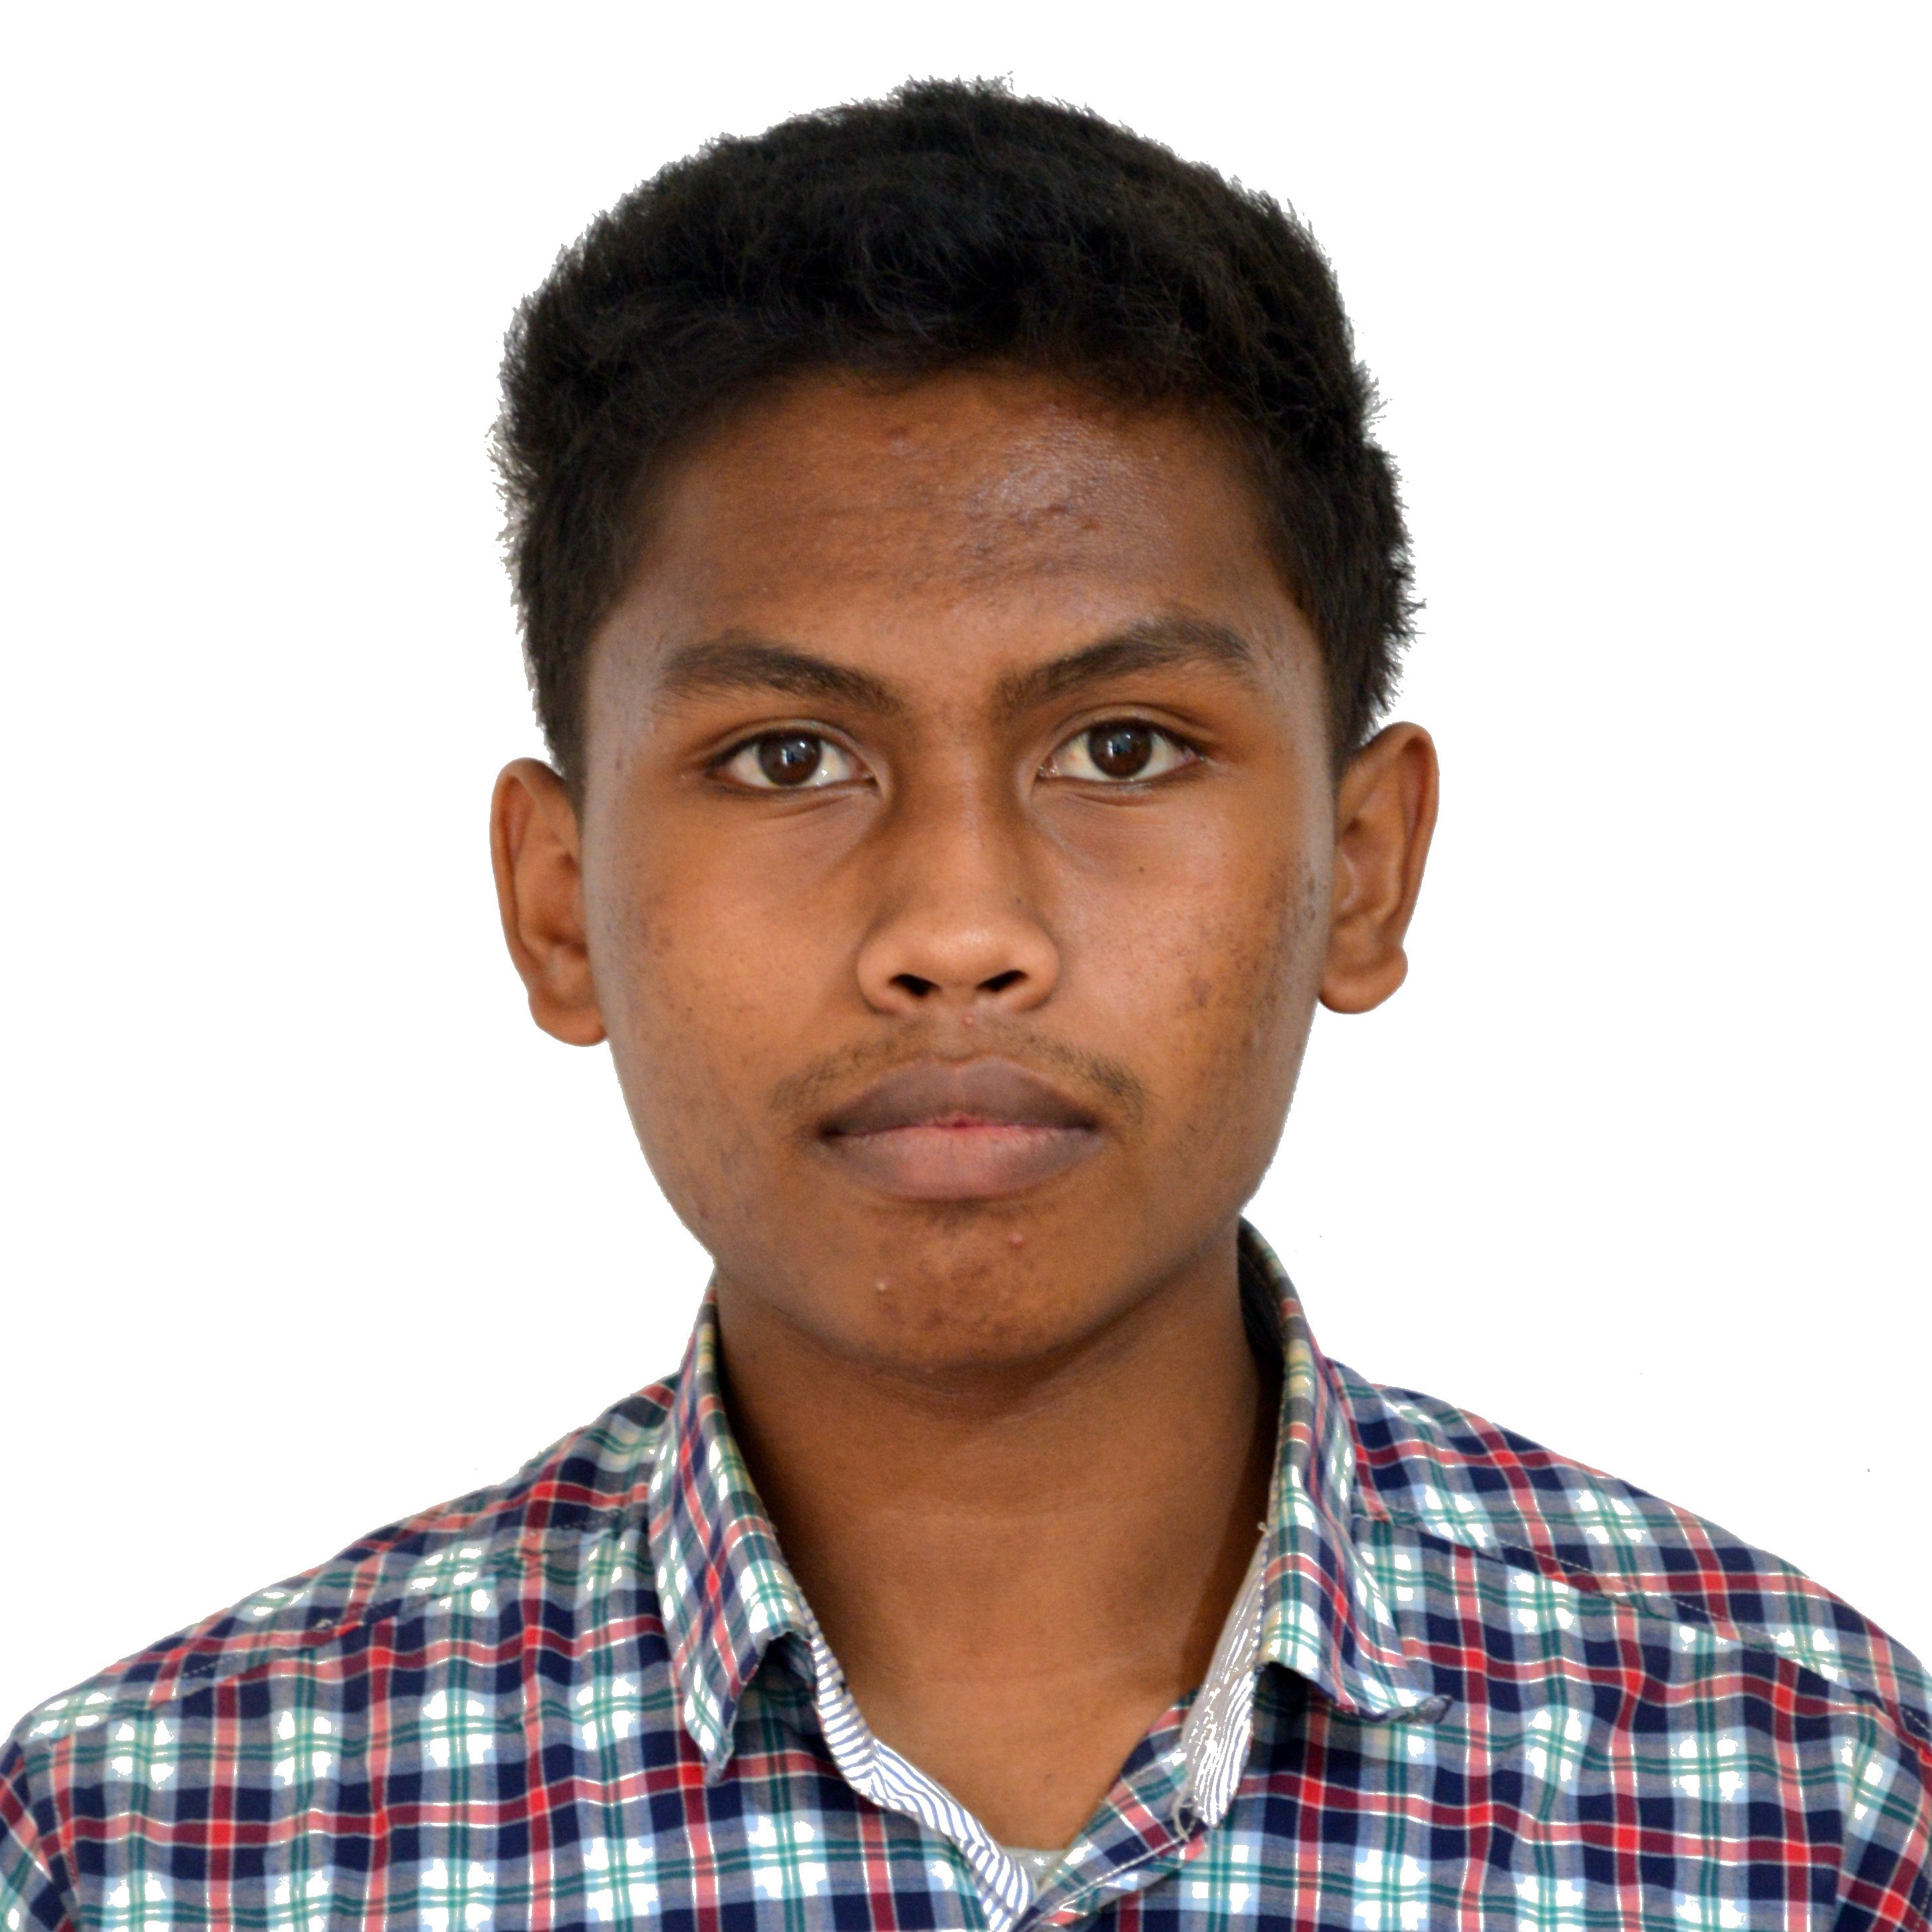
\includegraphics[width=3.5cm, height=3.5cm]{mypic.jpg}	
			\end{minipage}
			\section*{FORMATIONS ET DIPLOME}
			\begin{minipage}{\textwidth}
				\textbf{2024-2025:} Deuxième année de formation en Master professionnelle à l’École Nationale d'Informatique, Université de Fianarantsoa, parcours : Informatique générale.\\[0.5cm]
				\textbf{2023-2024:} Première année de formation en Master professionnelle à l’École Nationale d'Informatique, Université de Fianarantsoa, parcours : Informatique générale.\\[0.5cm]
				\textbf{2022-2023:} Obtention du diplôme de Licence professionnelle mention Bien à l’École Nationale d'Informatique, Université de Fianarantsoa, parcours : Informatique générale.\\[0.5cm]
				\textbf{2021-2022:} Deuxième année de formation en Licence professionnelle à l’École Nationale d'Informatique, Université de Fianarantsoa, parcours : Informatique générale.\\[0.5cm]
				\textbf{2020-2021:} Première année de formation en Licence professionnelle à l’École Nationale d'Informatique, Université de Fianarantsoa, parcours : Informatique générale.\\[0.5cm]
				\textbf{2019-2020:} Obtention du diplôme de Baccalauréat série D mention assez-bien au Lycée André Résampa Antsirabe.
			\end{minipage}
			\section*{STAGES ET EXPERIENCES PROFESSIONNELLES}
				\begin{minipage}{\textwidth}
       					 \textbf{11 juin 2024 au 4 novembre 2024:} Stage auprès de Nexitia technologies.
						\begin{itemize}
							\item Thème du stage: Application web Handeha voyage;
							\item Langages et outils: Java, spring boot, JavaScript, next js, Katappult, H2, UML.						
						\end{itemize}
       					 \textbf{Octobre 2023:} Projet à l’École Nationale d'Informatique.
						\begin{itemize}
							\item Thème du stage: Module de securité pour application spring boot et angular;
							\item Langages et outils: Java, spring boot, Angular, TypeScript, PostgreSQL, UML.						
						\end{itemize}       					 
					\textbf{19 octobre 2022 au 16 janvier 2023:} Stage auprès de la Paositra malagasy.
						\begin{itemize}
							\item Thème du stage: Application web pour la gestion des change;
							\item Langages et outils: Java, spring boot, Angular, TypeScript, PostgreSQL, UML.								
						\end{itemize}
					\textbf{Septembre 2022:} Projet à l’École Nationale d'Informatique.
						\begin{itemize}
							\item Thème du stage: Création d'une application mobile de gestion de cotisation de groupe;
							\item Langages et outils: Java, Android Studio.								
						\end{itemize}
					\textbf{8 mars 2021 au 7 juillet 2021:} Stage auprès du Ministère de l’Économie et de la Finance.
						\begin{itemize}
							\item Thème du stage: Application web pour la gestion des dossier du personnels de la Direction du Système d'Information;
							\item Langages et outils: Java, spring boot, Angular, TypeScript, PostgreSQL, UML.								
						\end{itemize} 
					\textbf{Avril 2021:} Projet à l’École Nationale d'Informatique.
						\begin{itemize}
							\item Thème du stage: Réalisation d’une application desktop de Gestion des heures complémentaires;
							\item Langages et outils: Php, MySQL, Ajax.								
						\end{itemize} 
					\textbf{Août 2020:} Projet à l’École Nationale d'Informatique.
						\begin{itemize}
							\item Thème du stage: Création d'une application desktop de gestion de stock;
							\item Langages et outils: C++, Qt Creator.								
						\end{itemize} 
   				\end{minipage}		
			\section*{CONNAISSANCES EN INFORMATIQUE}
			\begin{minipage}{\textwidth}
				\begin{itemize}
					\item \textbf{Systèmes d'exploitation:} Microsoft Windows, Linux;
					\item \textbf{Langages de Programmation:} Java, JavaScript, TypeScript, Python , C/C++;
					\item \textbf{Développement Web:} HTML5, CSS3, Tailwind CSS, React.js, Next.js, Angular, Node.js, Express.js;
					\item \textbf{Développement Backend:} Spring Framework, Node.js, Express.js;
					\item \textbf{Compétences en bases de données:} SQL, PostgreSQL, MySQL;
					\item \textbf{Outils de Gestion de Versions:} Git, GitHub, GitLab; 	
					\item \textbf{Outils DevOps:} Docker, Kubernetes, Jenkins, Ansible;
					\item \textbf{Outils de virtualisation:} Docker, VirtualBox, VMware, Vagrant; 	
					\item \textbf{Outils de tests et Assurance Qualité:} Jest, JUnit;
					\item \textbf{Outils et Méthodologies de Conception et Gestion de Projets Logiciels:} UML, Méthodologie Agile, 2TUP, MERISE, GRASP;
					\item \textbf{Outils de Documentation et de Préparation de Contenu:} LaTeX/TeX.	
				\end{itemize}

   			\end{minipage}		
			\section*{CONNAISSANCES LINGUISTIQUE}
			\begin{minipage}{\textwidth}
				\begin{center}
					\begin{tabularx}{\textwidth}{|c|X|X|X|X|}
						\hline
						\textbf{LANGUE} & \textbf{COMPREHENSION} & \textbf{LECTURE} & \textbf{PARLE} & \textbf{ECRIT}\\
						\hline
						Anglais & Bien & Bien & Assez-bien & Bien \\
						\hline
						Français & Bien & Bien & Bien & Bien\\
						\hline
					\end{tabularx}
				\end{center}
			\end{minipage}
			\section*{LOISIR ET CENTRES D'INTERET}
			\begin{minipage}{\textwidth}
				\begin{itemize}
					\item Musique;
					\item Podcast;
					\item Documentaires;
					\item Anime;
					\item Jeux video;
					\item	Lecture.
				\end{itemize}
			\end{minipage}	
			\chapter*{REMERCIEMENTS}
			\addcontentsline{toc}{chapter}{REMERCIEMENTS}	
			\begin{minipage}{\textwidth}
				\hspace{15pt} Avant toute chose, je tiens à remercier Dieu tout puissant et miséricordieux, qui m'a donné la force et la patience d'accomplir ce modeste travail.\\[0.5cm]
				Mes remerciements s’étendent également à :
				\begin{itemize}
					\item Monsieur HAJALALAINA Aimé Richard, Docteur HDR, Président de l'Université de Fianarantsoa, pour tout ce qu'il entreprend à l'Université;
					\item Monsieur MAHATODY Thomas, Docteur HDR, Directeur de l’École Nationale d'Informatique, qui nous à donné l'opportunité d'aller en stage pour ainsi permettre d’accroître nos compétences;
					\item Monsieur RANARISON Richard, Directeur Général de la Paositra Malagasy, pour son accueil et la confiance qu'il à accordée depuis mon arrivée dans l’établissement;
					\item Monsieur RATIARSON Venot, Maître de Conférences, mon encadreur pédagogique, pour ses conseils et échanges tout au long du stage;
					\item Madame RANDRIAMIHARISOA Rollande, mon encadreur professionnelle, qui m'a toujours guidée lors de la réalisation du projet;
					\item Monsieur RALAIVAO Jean Christian, Assistant d'Enseignement Supérieur et de Recherche,d’avoir accepté de présider la soutenance;
				 	\item Monsieur DIMBISOA William Germain, Docteur en Informatique, d'avoir accepté d'examiner mon présent travail;
					\item Toutes les personnels de la Paositra Malagasy, pour leurs accueils;
					\item Toutes les enseignants et les personnels de l’École Nationale d'Informatique qui se sont acharné à nous former durant l'année universitaire;
					\item Ma famille pour son soutien, que se soit moral, matériel ou financier.
				\end{itemize}
			\end{minipage}
			\newpage
			\tableofcontents
			\newpage
			\chapter*{NOMENCLATURE}
			\addcontentsline{toc}{chapter}{NOMENCLATURE}	
			\newpage
			\listoftables
			\newpage
			\listoffigures
			\newpage
			\newpage
			\pagenumbering{arabic}
			\setcounter{page}{1}
			\chapter*{INTRODUCTION GÉNÉRALE}
			\addcontentsline{toc}{chapter}{INTRODUCTION GÉNÉRALE}
			\begin{minipage}{\textwidth}
				\hspace{15pt} Avec sa biodiversité unique et sa richesse culturelle, Madagascar est une destination touristique de choix. Cependant, avec la demande pour des expériences de voyage personnalisées et accessibles en ligne en constante croissance, de nombreux opérateurs touristiques luttent pour obtenir la visibilité et les moyens nécessaires pour promouvoir efficacement leurs offres.\\

				\hspace{15pt} Malgré l'essor des plateformes de réservation en ligne, il demeure un besoin urgent d'une solution centralisée pour permettre aux opérateurs touristiques malgaches de partager leurs offres et aux voyageurs de réserver facilement leurs circuits ou séjours.\\

				\hspace{15pt} L'objectif de ce mémoire est de développer et de présenter "Handeha Voyage", une application web qui  facilite la mise en ligne des offres de circuits et de séjours par les opérateurs touristiques, simplifie le processus de réservation pour les utilisateurs et améliore la visibilité des opérateurs touristiques. Cette étude propose une solution novatrice qui répond directement aux défis rencontrés par les opérateurs touristiques et les voyageurs à Madagascar. En effet, l'application "Handeha Voyage" ne se contente pas de faciliter la réservation des voyages; elle redéfinit fondamentalement la manière dont les services touristiques sont présentés et consommés.\\

				\hspace{15pt} Ce mémoire abordera le processus de conception, de développement et de mise en œuvre de l'application "Handeha Voyage". Nous utiliserons des méthodes de conception et de modélisation adaptées, ainsi que des langages de programmation et frameworks appropriés, sans oublier un système de gestion de base de données solide. Tout cela sera orchestré selon une méthodologie de gestion de projet bien définie pour assurer une organisation optimale. Les limitations incluent le temps limité pour le développement complet de certaines fonctionnalités avancées, l'accès limité aux données et la difficulté à recueillir des retours d'expérience durant le développement.\\

				\hspace{15pt} Notre plan se subdivise en trois parties: dans un premier temps la présentation de l’École Nationale d'Informatique (ENI) suivie de celle de Nexitia Technology. Dans la deuxième partie, nous aborderons les analyses et la conception du projet. Enfin, la troisième partie portera sur la réalisation du projet avec les différents moyens et outils utilisés.
			\end{minipage}
			\part{PRESENTATION}
			\chapter{Présentation de l’Ecole Nationale d’Informatique}
			\section{Information d’ordre générale }
				\hspace{15pt} L’Ecole Nationale d’Informatique, en abrégé ENI, est un établissement d’enseignement supérieur rattaché académiquement et administrativement à l’Université de Fianarantsoa. Le siège de l’Ecole se trouve à Tanambao-Antaninarenina à Fianarantsoa. L’adresse pour la prise de contact avec l’Ecole est la suivante : Ecole Nationale d’Informatique (ENI) Tanambao, Fianarantsoa. Le numéro de sa boîte postale est 1487 avec le code postal 301. Téléphone : 034 05 733 36 ou 032 15 204 28. Son adresse électronique est la suivante : eni@eni.mg. Il dispose également d'un site web : \textbf{www.eni.mg}
			\section{Missions et historiques}
				\hspace{15pt} L’ENI se positionne sur l’échiquier socio-éducatif malgache comme étant le plus puissant secteur de diffusion et de vulgarisation des connaissances et des technologies informatiques. 

				Cette Ecole Supérieure peut être considérée aujourd’hui comme la vitrine et la pépinière des élites informaticiennes du pays.
	
				L’Ecole s’est constituée de façon progressive au sein du Centre Universitaire Régional (CUR) de Fianarantsoa.

				De façon formelle, l’ENI était constituée et créée au sein du (CUR) par le décret N° 83- 185 du 24 Mai 1983, comme étant le seul établissement Universitaire Professionnalisé au niveau national, destiné à former des techniciens et des Ingénieurs de haut niveau, aptes à répondre aux besoins et exigences d’Informatisation des entreprises, des sociétés et des organes implantés à Madagascar.

				           \begin{center}
						\begin{minipage}{\textwidth}
								\hspace{15pt} L’ENI a pour conséquent pour mission de former des spécialistes informaticiens compétents et opérationnels de différents niveaux notamment : 
				
								\begin{itemize}
									\item En fournissant à des étudiants des connaissances de base en informatique ;
									\item En leur transmettant le savoir-faire requis, à travers la professionnalisation des formations dispensées et en essayant une meilleure adéquation des formations par rapport aux besoins évolutifs des sociétés et des entreprises ;
									\item En initiant les étudiants aux activités de recherche dans les différents domaines des Technologies de l’information et de la communication (TIC).\\
								\end{itemize}
						\end{minipage}
					\end{center}

				L’implantation de cette Ecole Supérieure de technologie de pointe dans un pays en développement et dans une Province (ou Faritany) à tissu économique et industriel faiblement développé ne l’a pourtant pas défavorisée, ni empêchée de former des spécialistes informaticiens de bon niveau, qui sont recherchés par les entreprises, les sociétés et les organismes publics et privés sur le marché de l’emploi.

				La filière de formation d’Analystes Programmeurs a été mise en place à l’Ecole en 1983, et a été gelée par la suite en 1996, tandis que la filière de formation d’ingénieurs a été ouverte à l’Ecole en 1986.
				
				Dans le cadre du Programme de renforcement en l’Enseignement Supérieur (PRESUP), la filière de formation des Techniciens Supérieurs en Maintenance des Systèmes des informatiques a été mise en place en 1986 grâce à l’appui matériel et financier de la Mission Française de coopération auprès de l’Ambassade de France à Madagascar.

				Une formation pour l’obtention de la certification CCNA et / ou NETWORK +. Appelée « CISCO Networking Academy » a été créée à l’Ecole en 2002-2003 grâce au partenariat avec CISCO SYSTEM et l’Ecole Supérieure Polytechnique d’Antananarivo (ESPA). Cependant, cette formation n’avait pas duré longtemps. Une formation de troisième cycle a été ouverte à l’Ecole a été ouverte à l’Ecole depuis l’année 2003 – 2004 grâce à la coopération académique et scientifique entre l’Université de Fianarantsoa pour le compte de l’ENI et l’Université Paul Sabatier de Toulouse (UPST).
				
				 \begin{center}
					 \begin{minipage}{\textwidth}
	
						\hspace{15pt} Cette filière avait pour objectif de former certains étudiants à la recherche dans les différents domaines de l’Informatique, et notamment pour préparer la relève des Enseignants-Chercheurs qui étaient en poste. Pendant l’année 2007-2008, la formation en vue de l’obtention du diplôme de Licence Professionnelle en Informatique a été mise en place à l’ENI avec les deux options suivantes de formation :
						
						\begin{itemize}
							\item Génie Logiciel et base de Données.
							\item Administration des Système et réseaux.\\
						\end{itemize}
					\end{minipage}

				\end{center}
				
				La mise en place à l’Ecole de ces deux options de formation devait répondre au besoin de basculement vers le système Licence – Master – Doctorat (LMD). Mais la filière de formation des Techniciens Supérieurs en Maintenance des Systèmes Informatiques a été gelée en 2009. 
En vue de surmonter les difficultés de limitation de l’effectif des étudiants accueillis à l’Ecole, notamment à cause du manque d’infrastructures, un système de « Formation Hybride » a été mise en place à partir de l’année 2010. Il s’agit en effet d’un système de formation semi présentielle et à distance avec l’utilisation de la visioconférence pour la formation à distance. Le système de formation hybride a été ainsi créé à Fianarantsoa ainsi qu’Université de Toliara.

				\section{Organigramme institutionnel}

				\hspace{15pt} Cet organigramme de l’Ecole est inspiré des dispositions du décret N° 83-185 du 23 Mai 1983.

				L’ENI est administrée par un conseil d’Ecole, et dirigée par un directeur nommé par un décret adopté en conseil des Ministres.

				Le Collège des enseignants regroupant tous les enseignants-chercheurs de l’Ecole est chargé de résoudre les problèmes liés à l’organisation pédagogique des enseignements ainsi que à l’élaboration des emplois du temps.

				\begin{center}
					\begin{minipage}{\textwidth}
						\hspace{15pt} Le Conseil Scientifique propose les orientations pédagogiques et scientifiques de l’établissement, en tenant compte notamment de l’évolution du marché de travail et de l’adéquation des formations dispensées par rapport aux besoins des entreprises. Trois départements de formation caractérisent l’organigramme :
						\begin{itemize}
							\item Le département de formation théorique à l’intérieur de l’Ecole ;
							\item Le département de formation pratique pour la coordination et la supervision des stages en entreprise et des voyages d’études ;
							\item Le département de formation doctorale pour l’organisation de la formation de 3ème cycle. La figure \ref{fig:figure 1} présente l’organigramme actuel de l’Ecole.
						\end{itemize}
					\end{minipage}
				\end{center}

				\begin{figure}[h]
					  \centering
					  \includegraphics[width=\textwidth]{image4.png}
					  \caption{Organigramme institutionnel de l'ENI}
					  \label{fig:figure 1}
				\end{figure}
	
\end{document}	